\section*{UC1 - \textit{Login} dell'utente}

\begin{figure}[H]
    \centering
    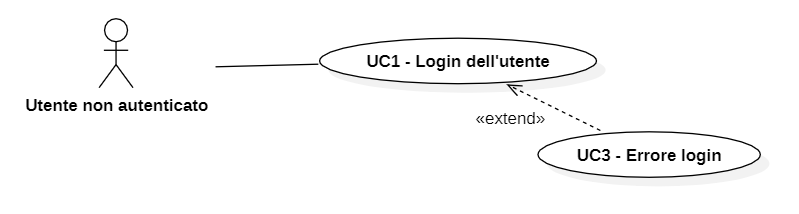
\includegraphics[scale=0.5]{usecase/uc1.png}
    \caption{UC1 - \textit{Login} dell'utente}
    \label{fig:uc1}
\end{figure}
\begin{itemize}
    \item \textbf{Attori}: Utente non autenticato;
    \item \textbf{Descrizione}: L'utente inserisce le proprie credenziali per accedere al sistema;
    \item \textbf{Precondizioni}: L'utente non è autenticato nel sistema;
    \item \textbf{Postcondizioni}: L'utente viene autenticato e reindirizzato alla \textit{dashboard} del sistema;
    \item \textbf{Flusso principale}:
    \begin{enumerate}
        \item L'utente naviga alla pagina di \textit{login};
        \item L'utente inserisce \textit{email} e \textit{password};
        \item Il sistema verifica le credenziali;
        \item Se le credenziali sono corrette, l'utente viene autenticato e reindirizzato alla \textit{dashboard}.
    \end{enumerate}
    \item \textbf{Estensioni}: UC3 - Visualizzazione errore in caso di \textit{login} non riuscito
\end{itemize}

\vspace{0.5cm}
\section*{UC2 - \textit{Logout} dell'utente}
\begin{itemize}
    \item \textbf{Attori}: Utente autenticato;
    \item \textbf{Descrizione}: L'utente può disconnettersi dal sistema;
    \item \textbf{Precondizioni}: L'utente è autenticato;
    \item \textbf{Postcondizioni}: L'utente viene disconnesso e reindirizzato alla pagina di \textit{login};
    \item \textbf{Flusso principale}:
    \begin{enumerate}
        \item L'utente clicca sul pulsante di \textit{logout};
        \item L'utente conferma la volontà di effettuare il \textit{logout};
        \item Il sistema disconnette l'utente;
        \item L'utente viene reindirizzato alla pagina di \textit{login}.
    \end{enumerate}
\end{itemize}

\vspace{0.5cm}
\section*{UC3 - Visualizzazione errore in caso di \textit{login} non riuscito}
\begin{itemize}
    \item \textbf{Attori}: Utente non autenticato;
    \item \textbf{Descrizione}: L'utente visualizza un messaggio di errore quando il \textit{login} fallisce;
    \item \textbf{Precondizioni}: L'utente ha inserito credenziali errate;
    \item \textbf{Postcondizioni}: Un messaggio di errore viene mostrato all'utente;
    \item \textbf{Flusso principale}:
    \begin{enumerate}
        \item L'utente inserisce credenziali errate;
        \item Il sistema verifica le credenziali;
        \item Il sistema visualizza un messaggio di errore indicando che il \textit{login} è fallito.
    \end{enumerate}
\end{itemize}

\vspace{0.5cm}  
\section*{UC4 - Visualizzazione lista progetti}
\begin{itemize}
    \item \textbf{Attori}: Utente autenticato;
    \item \textbf{Descrizione}: L'utente visualizza la lista di tutti i progetti disponibili;
    \item \textbf{Precondizioni}: L'utente è autenticato;
    \item \textbf{Postcondizioni}: La lista di progetti viene visualizzata;
    \item \textbf{Flusso principale}:
    \begin{enumerate}
        \item L'utente accede alla \textit{dashboard} del sistema;
        \item Il sistema recupera e visualizza la lista di tutti i progetti disponibili;
        \item L'utente può vedere il nome, la data di creazione ed il preset usato per la generazione dei progetti.
    \end{enumerate}
\end{itemize}

\vspace{0.5cm}  
\section*{UC5 - Ricerca e filtraggio dei progetti}
\begin{itemize}
    \item \textbf{Attori}: Utente autenticato;
    \item \textbf{Descrizione}: L'utente cerca e filtra i progetti utilizzando specifici criteri;
    \item \textbf{Precondizioni}: L'utente è autenticato e si trova nella dashboard di sistema;
    \item \textbf{Postcondizioni}: I progetti che soddisfano i criteri di ricerca e/o filtro vengono visualizzati;
    \item \textbf{Flusso principale}:
    \begin{enumerate}
        \item L'utente inserisce parole chiave e/o seleziona i filtri;
        \item Il sistema applica i filtri e visualizza i progetti corrispondenti.
    \end{enumerate}
\end{itemize}

\vspace{0.5cm}  
\section*{UC6 - Visualizzazione dei dettagli di un progetto singolo}
\begin{itemize}
    \item \textbf{Attori}: Utente autenticato;
    \item \textbf{Descrizione}: L'utente visualizza i dettagli di un progetto specifico selezionato dalla lista dei progetti;
    \item \textbf{Precondizioni}: 
    \begin{itemize}
        \item L'utente è autenticato;
        \item Il progetto selezionato è stato precedentemente creato dall'utente.
    \end{itemize}
    \item \textbf{Postcondizioni}: Il sistema mostra i dettagli del progetto selezionato, inclusi nome, descrizione, data di creazione, e tutti i capitoli che lo compongono;
    \item \textbf{Flusso principale}:
    \begin{enumerate}
        \item L'utente accede alla lista dei progetti salvati;
        \item L'utente seleziona un progetto dalla lista;
        \item Il sistema recupera i dati del progetto selezionato dal \textit{database};
        \item Il sistema mostra i dettagli del progetto in una pagina dedicata, inclusi:
        \begin{itemize}
            \item Nome del progetto;
            \item Descrizione del progetto;
            \item Data di creazione;
            \item Sezioni e contenuti specifici del progetto.
        \end{itemize}
    \end{enumerate}
\end{itemize}

\vspace{0.5cm}  
\section*{UC7 - Visualizzazione descrizione \textit{preset}}
\begin{itemize}
    \item \textbf{Attori}: Utente autenticato;
    \item \textbf{Descrizione}: L'utente visualizza la descrizione di un \textit{preset} disponibile;
    \item \textbf{Precondizioni}: L'utente è autenticato;
    \item \textbf{Postcondizioni}: La descrizione del \textit{preset} viene visualizzata;
    \item \textbf{Flusso principale}:
    \begin{enumerate}
        \item L’utente naviga nella pagina di creazione di un progetto;
        \item L'utente seleziona un \textit{preset} dalla lista di quelli disponibili;
        \item Il sistema visualizza la descrizione dettagliata del \textit{preset}.
    \end{enumerate}
\end{itemize}

\vspace{0.5cm}  
\section*{UC8 - Salvataggio di un \textit{preset} compilato}
\begin{itemize}
    \item \textbf{Attori}: Utente autenticato;
    \item \textbf{Descrizione}: L'utente salva un \textit{preset} parzialmente compilato come bozza;
    \item \textbf{Precondizioni}: L'utente è autenticato e deve aver iniziato a compilare un \textit{preset};
    \item \textbf{Postcondizioni}: Il \textit{preset} parzialmente compilato viene salvato come bozza;
    \item \textbf{Flusso principale}:
    \begin{enumerate}
        \item L'utente compila una parte del \textit{preset};
        \item L'utente clicca su "Salva bozza";
        \item Il sistema salva la bozza del \textit{preset} nel \textit{database}.
    \end{enumerate}
\end{itemize}

\vspace{0.5cm}  
\section*{UC9 - Visualizzazione lista bozze}
\begin{itemize}
    \item \textbf{Attori}: Utente autenticato;
    \item \textbf{Descrizione}: L'utente visualizza la lista di tutte le bozze disponibili;
    \item \textbf{Precondizioni}: L'utente è autenticato;
    \item \textbf{Postcondizioni}: La lista di bozze viene visualizzata;
    \item \textbf{Flusso principale}:
    \begin{enumerate}
        \item L'utente accede alla \textit{dashboard} del sistema;
        \item L'utente seleziona il pulsante di visualizzazione della lista di bozze;
        \item Il sistema recupera e visualizza la lista di tutte le bozze disponibili;
        \item L'utente può vedere il nome, la data di creazione ed il preset utilizzato per ogni bozza.
    \end{enumerate}
\end{itemize}

\vspace{0.5cm}  
\section*{UC10 - Ricerca e filtraggio delle bozze}
\begin{itemize}
    \item \textbf{Attori}: Utente autenticato;
    \item \textbf{Descrizione}: L'utente cerca e filtra le bozze utilizzando specifici criteri;
    \item \textbf{Precondizioni}: 
    \begin{itemize}
        \item L'utente è autenticato;
        \item L'utente si trova nella \textit{dashboard} di sistema ed ha selezionato il pulsante di visualizzazione della lista di bozze.
    \end{itemize}
    \item \textbf{Postcondizioni}: Le bozze che soddisfano i criteri di ricerca e/o filtro vengono visualizzate;
    \item \textbf{Flusso principale}:
    \begin{enumerate}
        \item L'utente inserisce parole chiave e/o seleziona i filtri;
        \item Il sistema applica i filtri e visualizza le bozze corrispondenti.
    \end{enumerate}
\end{itemize}

\vspace{0.5cm}  
\section*{UC11 - Generazione di un progetto}
\begin{figure}[H]
    \centering
    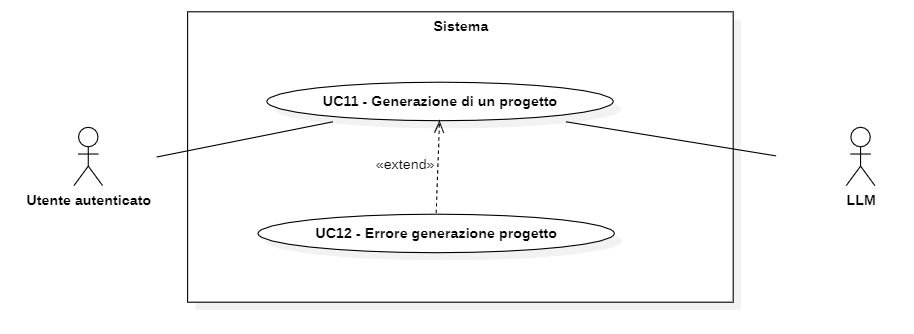
\includegraphics[scale=0.6]{usecase/uc11.png}
    \caption{UC11 - Generazione di un progetto}
    \label{fig:uc11}
\end{figure}
\begin{itemize}
    \item \textbf{Attori}: Utente autenticato, \gls{llm};
    \item \textbf{Descrizione}: L'utente avvia la generazione di un progetto utilizzando un \textit{preset};
    \item \textbf{Precondizioni}: 
    \begin{itemize}
        \item L'utente è autenticato;
        \item L'utente si trova nella pagina di creazione di un progetto ed ha selezionato un \textit{preset}.
    \end{itemize}
    \item \textbf{Postcondizioni}: Il progetto viene generato e l'utente vede le informazioni generate;
    \item \textbf{Flusso principale}:
    \begin{enumerate}
        \item L'utente compila nella sua interezza il \textit{preset} selezionato;
        \item L'utente richiede la generazione del progetto;
        \item Il sistema invia la richiesta al \gls{llm};
        \item Il \gls{llm} elabora la richiesta e genera il progetto;
        \item L'utente viene reindirizzato alla pagina di visualizzazione del progetto.
    \end{enumerate}
    \item \textbf{Estensioni}: UC12 - Visualizzazione errore generazione progetto
\end{itemize}

\vspace{0.5cm}
\section*{UC12 - Visualizzazione errore generazione progetto}
\begin{itemize}
    \item \textbf{Attori}: Utente autenticato;
    \item \textbf{Descrizione}: L'utente visualizza un messaggio di errore la generazione del progetto fallisce;
    \item \textbf{Precondizioni}: L'utente sta generando un progetto;
    \item \textbf{Postcondizioni}: Un messaggio di errore viene mostrato all'utente;
    \item \textbf{Flusso principale}:
    \begin{enumerate}
        \item L'utente invia la richiesta all'\gls{llm} per la generazione del progetto;
        \item \gls{llm} non riesce a generare il progetto richiesto;
        \item Il sistema visualizza un messaggio di errore indicando che la generazione del progetto è fallita.
    \end{enumerate}
\end{itemize}

\vspace{0.5cm}  
\section*{UC13 - Rigenerazione completa di un progetto}
\begin{figure}[H]
    \centering
    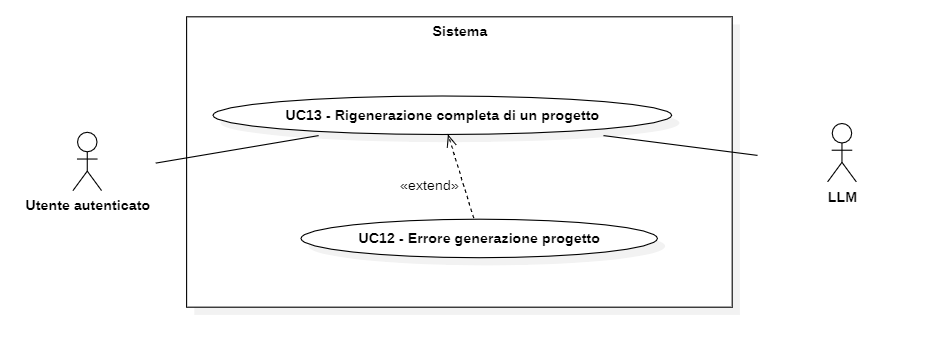
\includegraphics[scale=0.6]{usecase/uc13.png}
    \caption{UC13 - Rigenerazione completa di un progetto}
    \label{fig:uc13}
\end{figure}
\begin{itemize}
    \item \textbf{Attori}: Utente autenticato, \gls{llm};
    \item \textbf{Descrizione}: L'utente rigenera un intero progetto, sostituendo completamente il contenuto esistente;
    \item \textbf{Precondizioni}: 
    \begin{itemize}
        \item L'utente è autenticato;
        \item L'utente si trova nella pagina di visualizzazione del singolo progetto.
    \end{itemize}
    \item \textbf{Postcondizioni}: Il progetto viene completamente rigenerato;
    \item \textbf{Flusso principale}:
    \begin{enumerate}
        \item L'utente seleziona il pulsante di rigenerazione completa del progetto;
        \item Il sistema richiede all'utente l'inserimento di un prompt su cui si baserà la rigenerazione;
        \item L'utente richiede la rigenerazione del progetto;
        \item Il sistema invia la richiesta di rigenerazione al \gls{llm};
        \item Il \gls{llm} rigenera completamente il progetto;
        \item Il progetto rigenerato viene visualizzato all'utente.
    \end{enumerate}
    \item \textbf{Estensioni}: UC12 - Visualizzazione errore generazione progetto
\end{itemize}

\vspace{0.5cm}  
\section*{UC14 - Rigenerazione di un singolo capitolo di un progetto}
\begin{figure}[H]
    \centering
    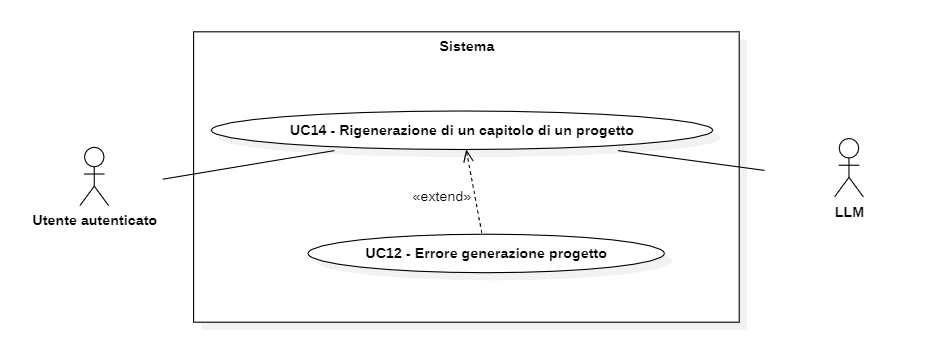
\includegraphics[scale=0.6]{usecase/uc14.png}
    \caption{UC14 - Rigenerazione di un singolo capitolo di un progetto}
    \label{fig:uc14}
\end{figure}
\begin{itemize}
    \item \textbf{Attori}: Utente autenticato, \gls{llm};
    \item \textbf{Descrizione}: L'utente rigenera un singolo capitolo del progetto, lasciando invariato il resto del progetto;
    \item \textbf{Precondizioni}: L'utente è autenticato e si trova nella pagina di visualizzazione del singolo progetto;
    \item \textbf{Postcondizioni}: Il capitolo selezionato viene rigenerato;
    \item \textbf{Flusso principale}:
    \begin{enumerate}
        \item L'utente seleziona il capitolo da rigenerare;
        \item Il sistema richiede all’utente l’inserimento di un \textit{prompt} su cui si baserà la rigenerazione;
        \item L’utente richiede la rigenerazione del capitolo;
        \item Il sistema invia la richiesta di rigenerazione al \gls{llm} per il capitolo selezionato;
        \item Il \gls{llm} rigenera solo il capitolo selezionato;
        \item Il progetto rigenerato viene visualizzato all'utente.
    \end{enumerate}
    \item \textbf{Estensioni}: UC12 - Visualizzazione errore generazione progetto
\end{itemize}

\vspace{0.5cm}  
\section*{UC15 - Eliminazione di un progetto}
\begin{itemize}
    \item \textbf{Attori}: Utente autenticato;
    \item \textbf{Descrizione}: L'utente elimina un progetto esistente;
    \item \textbf{Precondizioni}: L'utente è autenticato e si trova nella pagina di visualizzazione del singolo progetto;
    \item \textbf{Postcondizioni}: Il progetto viene eliminato dal sistema;
    \item \textbf{Flusso principale}:
    \begin{enumerate}
        \item L'utente seleziona il pulsante per l’eliminazione del progetto;
        \item L'utente conferma l'eliminazione del progetto;
        \item Il sistema elimina il progetto dal \textit{database}.
    \end{enumerate}
\end{itemize}

\vspace{0.5cm}  
\section*{UC16 - Visualizzazione del progetto in formato PDF}
\begin{itemize}
    \item \textbf{Attori}: Utente autenticato;
    \item \textbf{Descrizione}: L'utente visualizza il progetto generato in formato PDF;
    \item \textbf{Precondizioni}: L'utente è autenticato e si trova nella pagina di visualizzazione del singolo progetto;
    \item \textbf{Postcondizioni}: Il progetto viene visualizzato come PDF;
    \item \textbf{Flusso principale}:
    \begin{enumerate}
        \item L'utente seleziona il pulsante di visualizzazione del progetto in formato PDF;
        \item Il sistema mostra il progetto in formato PDF.
    \end{enumerate}
\end{itemize}

\vspace{0.5cm}  
\section*{UC17 - \textit{Download} del progetto in formato PDF}
\begin{itemize}
    \item \textbf{Attori}: Utente autenticato;
    \item \textbf{Descrizione}: L'utente scarica il progetto in formato PDF;
    \item \textbf{Precondizioni}: L’utente si trova nella pagina di visualizzazione del singolo progetto ed ha selezionato il pulsante di visualizzazione del PDF;
    \item \textbf{Postcondizioni}: Il progetto in formato PDF viene scaricato nel dispositivo dell'utente;
    \item \textbf{Flusso principale}:
    \begin{enumerate}
        \item L’utente seleziona il pulsante di \textit{download} del progetto in formato PDF;
        \item L'utente scarica il progetto in formato PDF.
    \end{enumerate}
\end{itemize}

\vspace{0.5cm}  
\section*{UC18 - Visualizzazione delle versioni precedenti di un progetto}
\begin{itemize}
    \item \textbf{Attori}: Utente autenticato;
    \item \textbf{Descrizione}: L'utente visualizza una lista delle versioni precedenti di un progetto selezionato e può accedere ai dettagli di una specifica versione;
    \item \textbf{Precondizioni}: L'utente è autenticato e il progetto selezionato ha almeno due versioni salvate;
    \item \textbf{Postcondizioni}: 
    \begin{itemize}
        \item Il sistema mostra la lista delle versioni precedenti del progetto, inclusi dettagli come numero di versione e data di creazione;
        \item L'utente può selezionare una versione specifica e visualizzarne i dettagli.
    \end{itemize}
    \item \textbf{Flusso principale}:
    \begin{enumerate}
        \item L'utente accede alla pagina dei dettagli di un progetto;
        \item L'utente seleziona la versione del progetto;
        \item Il sistema recupera e mostra una lista delle versioni precedenti del progetto, con i seguenti dettagli:
        \begin{itemize}
            \item Numero di versione;
            \item Data di creazione.
        \end{itemize}
        \item L'utente seleziona una specifica versione dalla lista;
        \item Il sistema mostra i dettagli della versione selezionata, inclusi i contenuti del progetto in quella versione.
    \end{enumerate}
\end{itemize}

\vspace{0.5cm}  
\section*{UC19 - Rimozione di capitoli non necessari da un progetto}
\begin{itemize}
    \item \textbf{Attori}: Utente autenticato;
    \item \textbf{Descrizione}: L'utente rimuove uno o più capitoli non necessari da un progetto per semplificarne la struttura o adattarlo a nuove esigenze;
    \item \textbf{Precondizioni}: 
    \begin{itemize}
        \item L'utente è autenticato;
        \item Il progetto contiene capitoli modificabili o rimovibili.
    \end{itemize}
    \item \textbf{Postcondizioni}: 
    \begin{itemize}
        \item Il sistema aggiorna la struttura del progetto eliminando i capitoli selezionati;
        \item La versione aggiornata del progetto è salvata nel sistema.
    \end{itemize}
    \item \textbf{Flusso principale}:
    \begin{enumerate}
        \item L'utente accede alla pagina di visualizzazione di un progetto;
        \item L'utente seleziona l'opzione "Gestione capitoli";
        \item Il sistema mostra la lista dei capitoli attualmente presenti nel progetto;
        \item L'utente seleziona uno o più capitoli che desidera rimuovere;
        \item L'utente conferma l'operazione di rimozione;
        \item Il sistema elimina i capitoli selezionati e aggiorna il progetto.
    \end{enumerate}
\end{itemize}